\documentclass{standalone}
\usepackage{amsmath}
\usepackage{amssymb}
\usepackage{tikz}
\usetikzlibrary{arrows.meta,positioning}

\definecolor{DataOrange}{RGB}{255,209,166}
\definecolor{ProcessTeal}{RGB}{160,214,209}

\begin{document}
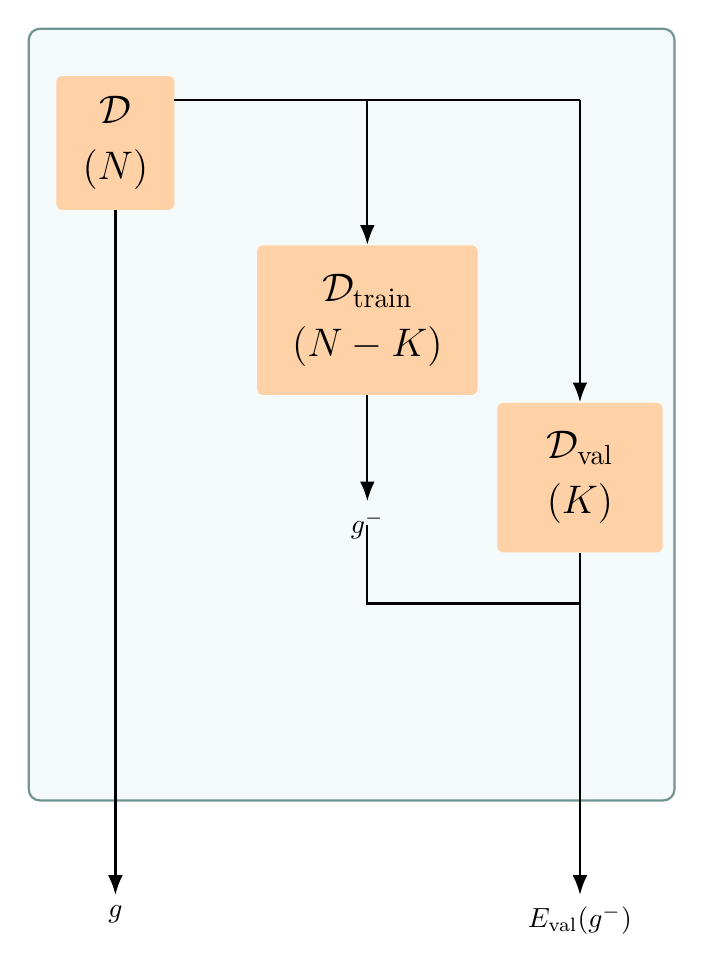
\begin{tikzpicture}[
  font=\sffamily,
  box/.style={
    rectangle,
    rounded corners=2pt,
    fill=DataOrange,
    draw=none,
    align=center,
    font=\Large
  },
  arrow/.style={-{Latex[length=2.5mm]}, thick},
  wire/.style={thick},
  label/.style={font=\normalsize}
]

  \draw[ProcessTeal!70!black, thick, rounded corners=4pt, fill=ProcessTeal!12]
    (0.4,1.8) rectangle (8.6,11.6);

  \node[box, minimum width=1.5cm, minimum height=1.7cm] (dataset) at (1.5,10.15) {$\mathcal{D}$\\[2pt]$(N)$};
  \node[box, minimum width=2.8cm, minimum height=1.9cm] (train) at (4.7,7.9) {$\mathcal{D}_{\text{train}}$\\[2pt]$(N-K)$};
  \node[box, minimum width=2.1cm, minimum height=1.9cm] (val) at (7.4,5.9) {$\mathcal{D}_{\text{val}}$\\[2pt]$(K)$};

  \coordinate (DExit)     at (2.25,10.7);
  \coordinate (TopRight)  at (7.4,10.7);
  \coordinate (TopBranch) at (4.7,10.7);
  \coordinate (GMinusTurn) at (4.7,4.3);
  \coordinate (JoinPoint)  at (7.4,4.3);

  \draw[wire]  (DExit) -- (TopRight);
  \draw[arrow] (TopRight)  -- (val.north);
  \draw[arrow] (TopBranch) -- (train.north);

  \draw[arrow] (dataset.south) -- (1.5,0.6) node[below, label] {$g$};

  \draw[arrow] (train.south) -- (4.7,5.6) node[below, label] {$g^-$};

  \draw[wire] (4.7,5.3) -- (GMinusTurn) -- (JoinPoint);
  \draw[wire]  (val.south) -- (JoinPoint);
  \draw[arrow] (JoinPoint) -- (7.4,0.6) node[below, label] {$E_{\text{val}}(g^-)$};

\end{tikzpicture}
\end{document}
